\chapter{Spherical SfM}
\lhead{\chaptername~\thechapter. \emph{Spherical SfM}}
In this chapter, we describe the pipeline that we designed to create a dense 
point cloud from a set of equirectangular images.
In Section~\ref{sec:pipeline_pose_estimation}, we describe the first phase of our
pipeline: the selection of the frames from the input sequence and the estimatation of
the camera trajectory. In Section~\ref{sec:pipeline_densification}, we describe 
our densification algorithm for equirectangular images.
Fig.~\ref{fig:pipeline_overview} shows a coarse visualization of these two macro parts of the 
pipeline. Pose estimation and densification are 
expanded further in Figures~\ref{fig:sfm_block} and \todo{aggiungere ref a immagine}.

\begin{figure}
    \centering
    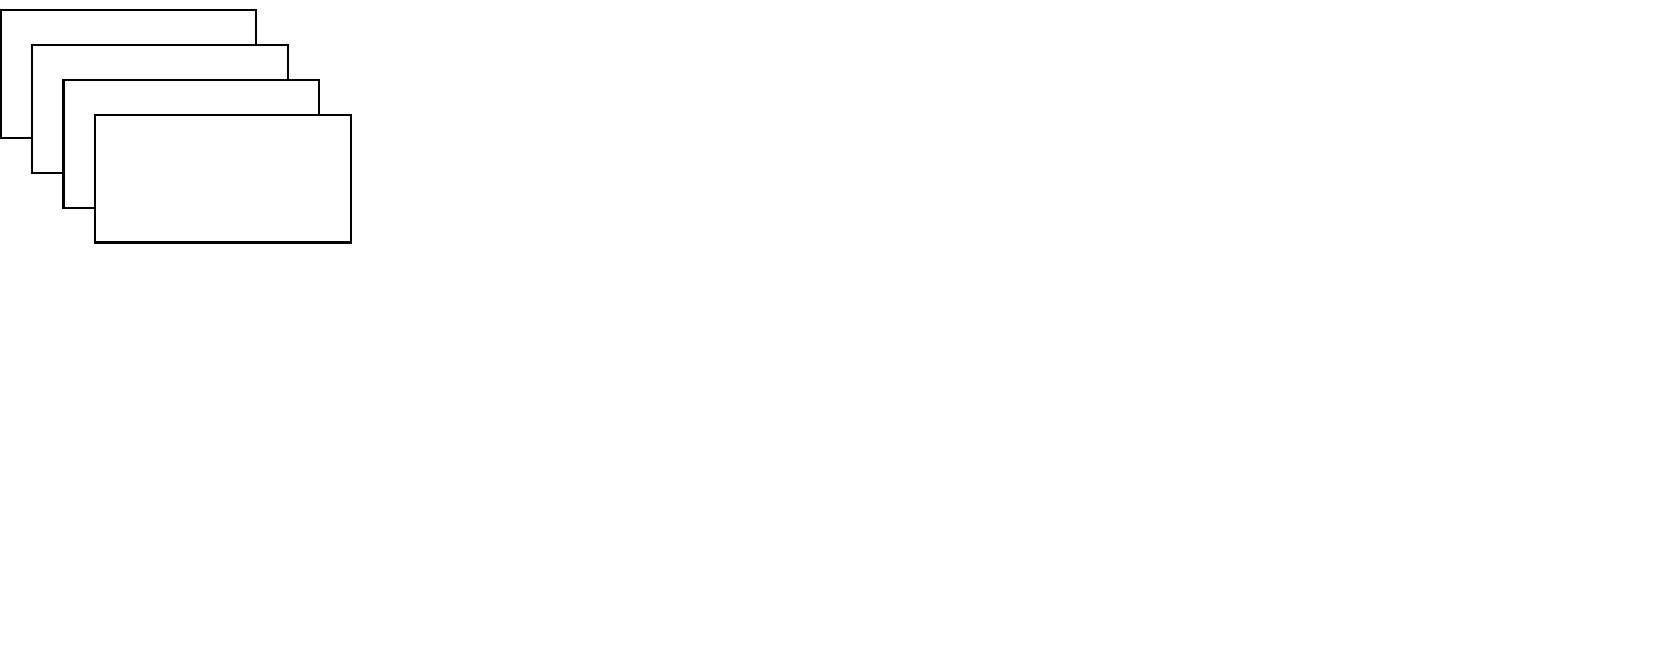
\includegraphics[width=0.8\linewidth]{img/pipeline_overview.pdf}
    \caption{The proposed SfM pipeline for spherical images: the frame selector chooses which frames are 
    relevant for the next processing steps; the pose estimation phase returns the cameras' 
    poses and the sparse points cloud; the densification step uses 
    the input images and the previous camera's poses to generate a dense
    reconstruction of the environment. See Figures\ref{fig:sfm_block} and ....}
	\label{fig:pipeline_overview}
\end{figure}

\section{Pose Estimation}
\label{sec:pipeline_pose_estimation}
The cameras' poses estimation phase is similar to the classical visual 
odometry pipeline. The main differences lie in the variables' format and in 
the details concerning the procedures used.
For each new frame (in the equirectangular representation), we locate the
SURF keypoints~\cite{bay2006surf}; we consider those keypoints whose inclination angle is in the range $[-60\degree; +60\degree]$. This is because the poles may be affected by large 
distortions, thus robust matches outside this interval are rare.
Then, we look for matches in the last two frames. A filter performs a 
statistical analysis on the correspondences found and decides whether the frame 
is suitable for a robust pose estimation or not (in this case the frame is 
discarded).

If the frame is kept, its matches with the previous ones are converted
and used for the essential matrix ($E$) estimation. Once $E$ is computed, 
it can be decomposed into the \([R|t]\) form; where $R$ is a rotation matrix 
and $\myvec{t}$ is a translation vector up to an unknown scale factor.

The relative scale can be estimated by using world points that have been 
triangulated through matches and the frame considered in the previous pipeline 
iteration.

Then, the pose of each camera can be described as the composition of the 
motions between each view pair. We perform a bundle adjustment for the last five 
poses in order to reduce the effect of drift (see Section~\ref{sec:vo_problem}
for details about drift).

After the processing of all images, a final bundle adjustment step is performed. 
This optimizes every camera pose (previously estimated) in order to reduce drift error further.

Figure~\ref{fig:camera_model} shows the coordinate system used in our pipeline: the X-axis points right, the Y-axis points down, and the Z-axis points forward. We consider the spherical image divided into two hemispheres: front and back. We call \textit{frontal points} the image points such that the $z$ component is positive, otherwise we use the term \textit{rear points}.
When we need to express spherical coordinates, we use the same angles as shown in 
Figure~\ref{fig:camera_model}:
the angle between the Z-axis and the projection of $m$ on the XZ-plane in 
the clockwise direction is the longitude angle ($\lambda$), and the angle 
between the negative Y-axis and the same projection of $m$ is the latitude 
angle ($\phi$).

\textbf{Francesco's note: il flow chart non ha un begin vero, martedi' ti spiego come cambiare il flow chart}
\todo[inline]{Ancora da correggere.}
\begin{figure}
	\centering
	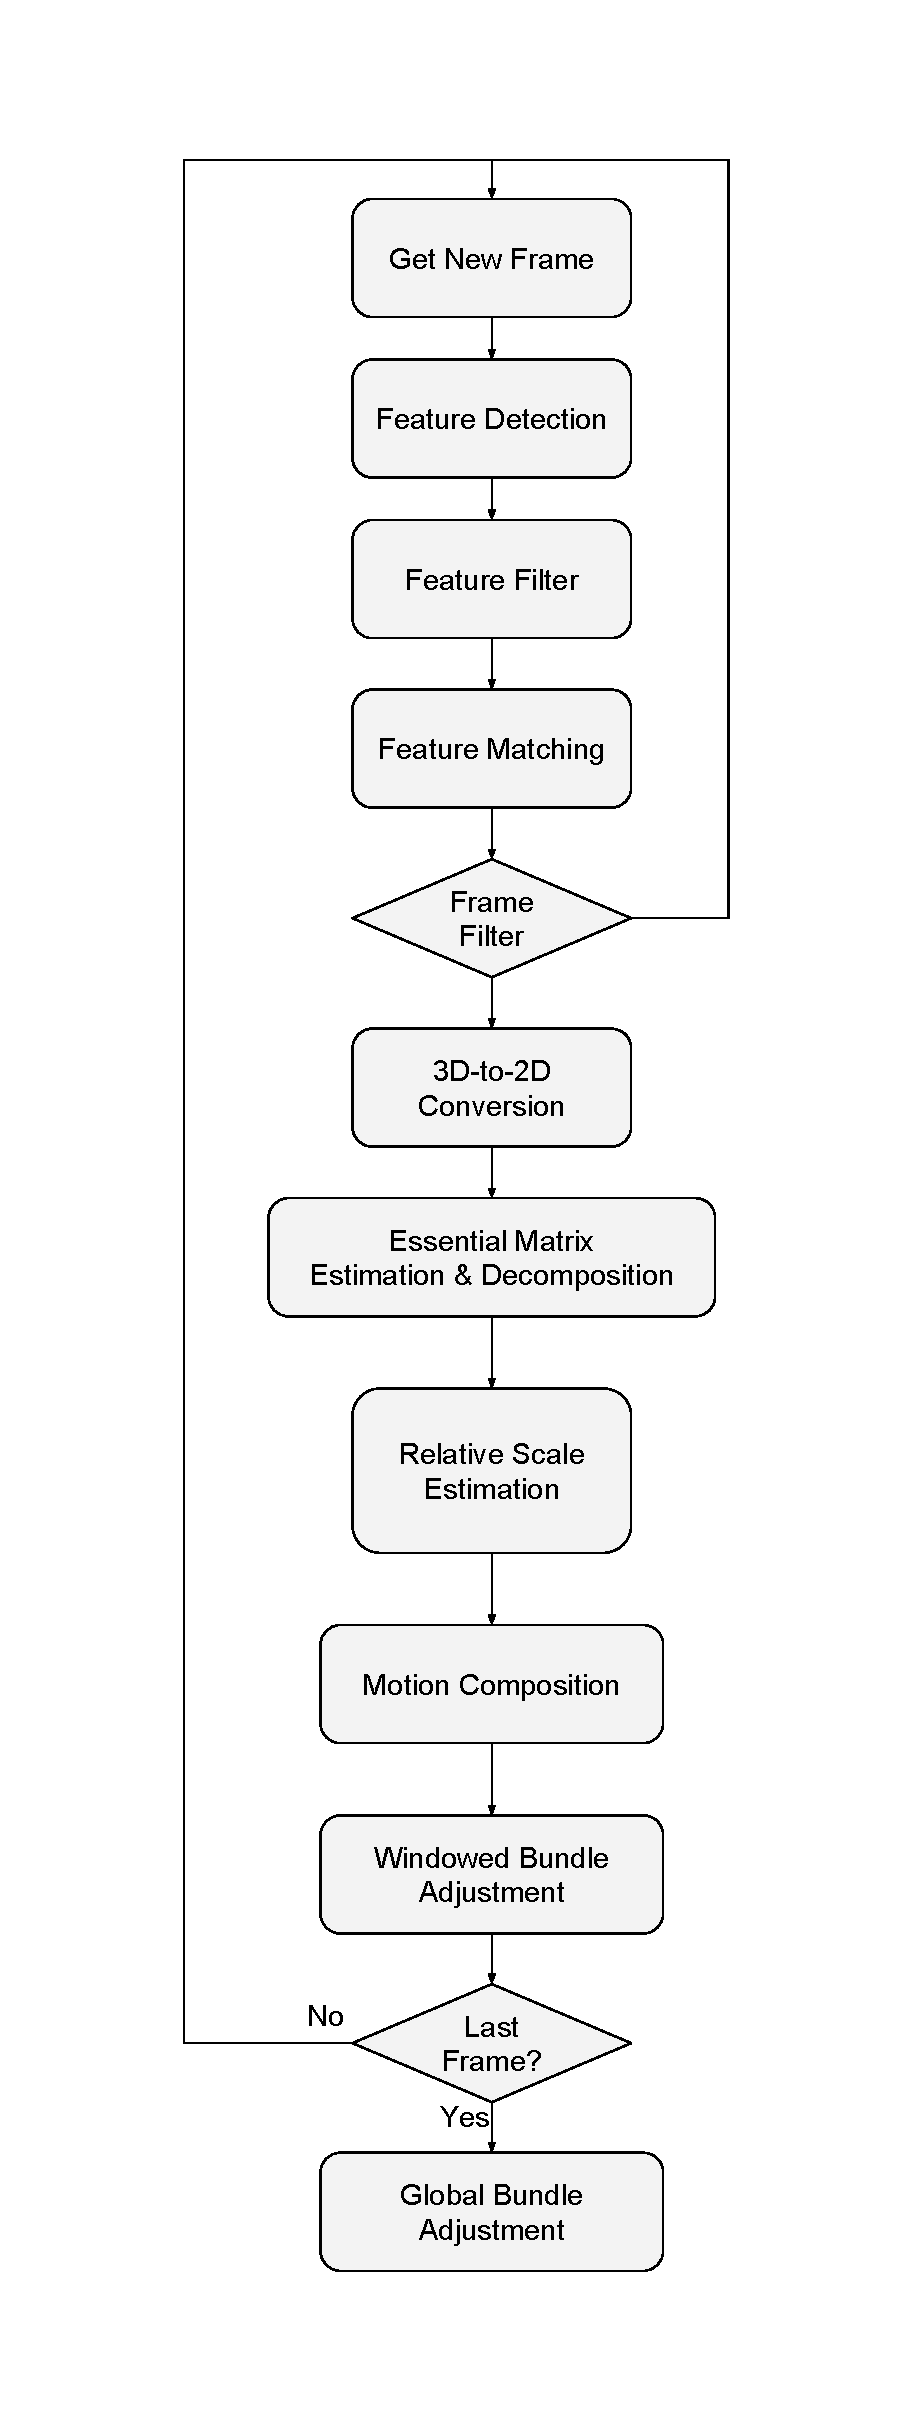
\includegraphics[width=0.5\linewidth]{img/sfm_block.pdf}
	\caption{The flow chart of steps performed in the pose estimation 
	phase of our SfM pipeline.}
	\label{fig:sfm_block}
\end{figure}

\subsection{Keypoints and Features Extraction}
In Section~\ref{sec:pipeline_pose_estimation}, we have introduced the need for 
features detection in order to find correspondences among the image pairs.
In our pipeline, we use SURF features and descriptors~\cite{bay2006surf},
which is a blob detector partly inspired by SIFT~\cite{lowe1999object}.
SURF performs convolution on integral images with box filters in order to 
compute the Hessian matrix in scale space.
This descriptor exploit keypoint's neighbourhood response to the Haar wavelet.
SURF, as SIFT, is patented. However, it can be used freely in non-commercial
applications and for academic research.
An implementation of the SURF detector is available in the MATLAB's Computer 
Vision Toolbox, and we employed it in our pipeline.

\subsection{Keypoints Filtering}
The equirectangular representation for spherical images introduces significant 
distortions around poles. Keypoints in those areas 
are unlikely to match reliably with other points in a consecutive view, therefore they are discarded.
Besides, in our experiments setup, the North and South poles typically point 
upward and downward respectively, while most of the matches useful for pose 
estimation comes from the sides of the camera. Therefore, the removal of interesting 
points near the poles does not affect the final result.

\subsection{Features Matching}\label{subsec:feature_matching}
The matching strategy, which we carried out for equirectangular images, is the same one 
adopted with standard images: two keypoints matches if the distance between 
their descriptors is less than a given threshold
(see Section~\ref{subsec:motion_estimation} for the 2D-to-2D features matching
approach). Ambiguous matches 
are discarded if the ratio between the distances to the two closest matches is 
above a maximum.
We enforce matching robustness by exploiting the fact that the correspondences are unique; i.e., only one feature in the first image can match with another one in the second image. This is achieved with two passes of the matching procedure. During the 
first pass, each feature in the first images is checked for correspondences in
the second image. In the second pass, each feature of the second image that 
has at least one correspondence in the first image is checked to see what 
interesting point of the first image it corresponds to and the match with the
highest confidence is kept.

\subsection{Matches Filter}
In this step of the pipeline, matches are analyzed in order to decide 
whether a frame has to be kept because it is useful for motion estimation or
not.
%
We assume that the scene to capture is static; i.e., no moving objects such as cars or people. In this case, the apparent movement of corresponding objects in different views is caused by the camera motion only.
%
The filter computes the disparity between every match found in two views; i.e., 
it compares the median of the 20\% of matches with the highest 
disparity value with a threshold. If such median is above 
the threshold, the frame is kept for further processing in the pipeline, 
otherwise it is discarded.
%
The reason because we consider the correspondences with the greatest disparity is 
because, when the camera rotation is limited, the points that move very little 
in consecutive views are typically far. The selection of these points for motion 
estimation can be counter-productive because they can easily produce numerical 
errors. 

\subsection{Keypoints Conversion}
\label{sec:keypoints_conversion}
%
This step converts the keypoint format of equirectangular images to a new one, which is
suitable for estimating $E$.
%
First, the latitude and longitude coordinates of each feature point are 
extracted from the 2D mapping according to Equation~\ref{eq:ll2Cartesian_first}.
This equation returns spherical coordinates for each feature point. 
Then, we can convert each of them to its cartesian format using Equation~\ref{eq:ll2Cartesian_second}. 
%
In order to estimate $E$ for each view pair, we use Equation~\ref{eq:epipolar_equation}, which was
introduced by Longuet-Higgins~\cite{longuet1981computer}.
The point coordinates, which we obtain from Equation~\ref{eq:ll2Cartesian_first} and
Equation~\ref{eq:ll2Cartesian_second}, do not need normalisation because there
is no intrinsic parameter for the full spherical camera model.

In order to exploit functions to estimate $E$ available in the MATLAB's Computer Vision Toolbox, we need to perform an additional step, because this toolbox's routines deal with standard 2D perspective images. Therefore, they expect 
2D points since the input arguments are image points. However, our camera provides image points on a sphere, and so are 3D points. To account for this problem we point out that we can multiply the points $\myvec{p}$ and $\myvec{p}'$ by two 
scalars ${\lambda}$ and ${\lambda}'$ and the equation is still valid. Thus, we obtain

\begin{equation*}
\lambda^\prime{\mathbf{p}^\prime}^\top E\lambda\mathbf{p} = 0 \text{.}
\end{equation*}

Therefore, we divide the 3D points obtained from the spherical images by their 
3rd component, discard it, and use the resulted 2D points as input for the 
MATLAB's function {\tt estimateEssentialMatrix}, which estimates $E$.

\begin{figure}
    \centering
    \def\svgwidth{0.8\columnwidth}
    \input{img/featurepoints_conversion.pdf_tex}
    \caption{A top view representation of the full spherical image's 
    different portions.
    The feature points that lie on the blue and green parts of the sphere are kept and,
    after the conversion described in Section~\ref{sec:keypoints_conversion},
    they are used for $E$ estimation. On the other hand, the points that lie
    on the red portions of the sphere are just discarded.
    Both the frontal point $p$ and the rear point $q$ are projected in $m$.}
	\label{fig:sphere_division}
\end{figure}

\subsubsection{Division by 3rd component vs. Projection}
%Our method (division by the 3rd component of the vectors) and the perspective projection on a plane for feature points conversion have some important differences.
%
Kangni et al.~\cite{kangni2007orientation} converted the 
feature points extracted from spherical images to their projected images on a 
planar surface and used traditional techniques to estimate the camera poses.
%
Even though our method is very similar to Kangni et al., there are some differences.
\textbf{Francesco's note: CHE DIFFERENZE???}\todo[inline]{le differenze sono quelle che
descrivo di seguito: maggior numero di parameteri in gioco e l'impossibilita'
di usare front e rear con un'unica proiezione. Meglio se qui metto una lista delle 
differenze e poi lascio il resto di questa sezione come descrizione dettagliata?}
\todo{si metti una lista!}
Projecting a point means that we have to deal with perspective geometry and its
parameters (e.g., pixel size or density), the principal point coordinates, 
focal length, image size, etc.

We can think to our method as a simplified perspective projection in which
$f_x$ and $f_y$ are both set to 1, and $u_0$ and $v_0$ are 0.
The main difference between our method and a standard projection is that, if we
just divide each feature point by its z-coordinate, we do not need to 
differentiate between frontal and rear points.
Figure~\ref{fig:sphere_division} shows how both the frontal point, $p$, and the 
rear one, $q$, are projected to the same point $m$ on the image plane.
This is not an issue, on the contrary, this helps the estimation of $E$ because 
it adds more redundant data to the input.

Note that we need to take care of numerical errors only: if we divide by a 
small number, the result is affected by a large error. Therefore, we
set a minimum value for the absolute value of the $z$-coordinate a feature point must 
have in order to be used in motion estimation. If the $z$ of a
feature point is below the threshold, we discard the point.
%
We called this threshold parameter $z_{min}$.
In Figure~\ref{fig:sphere_division}, the red area is not taken into account 
during motion estimation because the value of the magnitude of the 
$z$-coordinate of points there 
is below $z_{min}$.
%
Selecting points whose last component is above a certain threshold is 
equivalent to discarding those points that do not fit in the image plane
when projecting them. More details on this theory can be found in the
Szeliski's book~\cite{szeliski2010computer} and Hartley and Zisserman's
books~\cite{Hartley2004}.

\subsection{Essential Matrix Estimation and Decomposition}\label{subsec:essential_estimation}
As we have described in the previous section, $E$ is estimated 
by the function {\tt estimateEssentialMatrix} of the MATLAB's 
Computer Vision Toolbox.
We use both frontal and rear image points for this estimation because
more correspondences between image pairs produces more accurate results.

Once $E$ is estimated, we need to decompose it in the 
\( [R|\myvec{t} ] \) form. This is again performed by a Computer Vision 
Toolbox's function; i.e., {\tt relativeCameraPose}.
The inputs for this function are $E$, the camera parameters, and matches found in the last two images.
We need these matches because there are four possible decompositions for $E$. Each of these represents a different physical configuration for the cameras and world points.
In order to decide which decomposition is correct, in general, it is necessary to reproject the matches in their corresponding world points according to each 
decomposition and selects the one that reprojects most of the correspondences in 
front of both cameras.
Since our cameras are full spherical and the image points belong to the 
rear hemisphere too, we need to pay attention to use the frontal points only to resolve this ambiguity. 
The reduced number of matching points for the input of the 
{\tt relativeCameraPose} function does not compromise the accuracy of the pose 
estimated, since those matches are used only to choose the 
correct decomposition.

As we demonstrate with the experiments in Section~\ref{subsec:essential_test}, we obtain better
results if we call the essential matrix estimation routine until it satisfies
a minimum threshold of valid points ratio. This ratio is returned by the
estimation routine itself and represent the fraction of points whose
reprojection error, according to the estimated essential matrix,
is below a given threshold and thus are
considered inliers by the RANSAC algorithm.

\subsection{Relative Scale Estimation}
Every relative motion between two views can only be estimated up to an unknown 
scale factor. Indeed the scale affects just the translation, but it has to 
be computed in order to create a coherent set of camera poses.
We obtain the relative scale using 
Equation~\ref{eq:relative_scale}~\cite{scaramuzzaVisualOdometryI}.
This equation provides as many results as 3D points present in the last three
frames. In order to compensate for the effects of outliers, we take the 
median.

\subsection{Motion Composition}
Once we have estimated the relative motion between two views, we use 
Equation~\ref{eq:motion_composition} to compute the new camera pose $C_n$ from 
the last estimated pose $C_{n-1}$ and the results $R_{n}$ and $t_n$ obtained 
from the decomposition of $E$.
We set the first orientation, $R_0$, to $I$ and the magnitude of the first 
translation, $t_0$, to 1.

\subsection{Windowed Bundle Adjustment}\label{subsec:windowed_ba}
Since every local motion estimation is inevitably affected by error, the overall 
camera's path estimation tends to deviate from the real trajectory.
In order to reduce the drift and to get closer to a better starting point 
for the final bundle adjustment, we perform a bundle adjustment over the last five poses every time we process a new frame.
This local optimization step on the most recent subset of frames is called
\textit{Windowed Bundle Adjustment}.

The bundle adjustment tries to reduce the sum of reprojection errors by changing the
world points, and camera positions. 
We keep the camera poses associated with the two oldest frames of the window 
fixed in order to prevent the adjustment from modifying the reconstruction's 
scale. This constraint also helps reducing the number of variables for the 
adjustment.

\subsection{Global Bundle Adjustment}
When all the views have been processed, we perform a final bundle adjustment 
step, in order to further reduce drift. Again, the first two poses are fixed in 
order to keep the relative scale.

\section{Point Cloud Densification}
\label{sec:pipeline_densification}
In this chapter, we describe our pipeline's multi-view reconstruction step.
Its goal is to create a dense point cloud from the sparse one that we obtain
from the previous pose estimation step.
As we said in Section~\ref{sec:mvs}, the approach we followed for the
reconstruction is based on merging several depth maps that have been computed
from a set of consecutive image pairs.
In order to compute the disparity maps, we have to transform each image pair
through the \emph{rectification} transformation, i.e. the images have to be
transformed as they were taken from cameras whose X-axes were aligned along the
baseline and whose Z-axes lay on the same plane.
The purpose of the rectification is to speed up the computation and reduce the 
complexity of the disparity estimation step; it also helps by
reducing the wrong correspondences we would find with
non-rectified image pairs. Section~\ref{subsec:rectification} describes the
rectification for spherical cameras.
Once we have rectified image pairs, we use a block-matching algorithm to create
the disparity map. In Section~\ref{subsec:disparityMap}, we describe
the specific correspondence metric we use and the details about our own
solution to reduce the effect of the equirectangular image representation distortions
(Section~\ref{subsubsec:patch_creation}).
Sections~\ref{subsec:triangulation} and \ref{subsec:merging_worldPoints}
describe how we compute the 3D points' coordinates and express these points in
a unique coordinate system.
Figure~\ref{fig:densification_fc} shows all the steps needed to
create a dense point cloud from the previously estimated camera poses and
corresponding views.
In this thesis, we use the naming convention shown in
Figure~\ref{fig:naming_convention}.

\begin{figure}
	\centering
	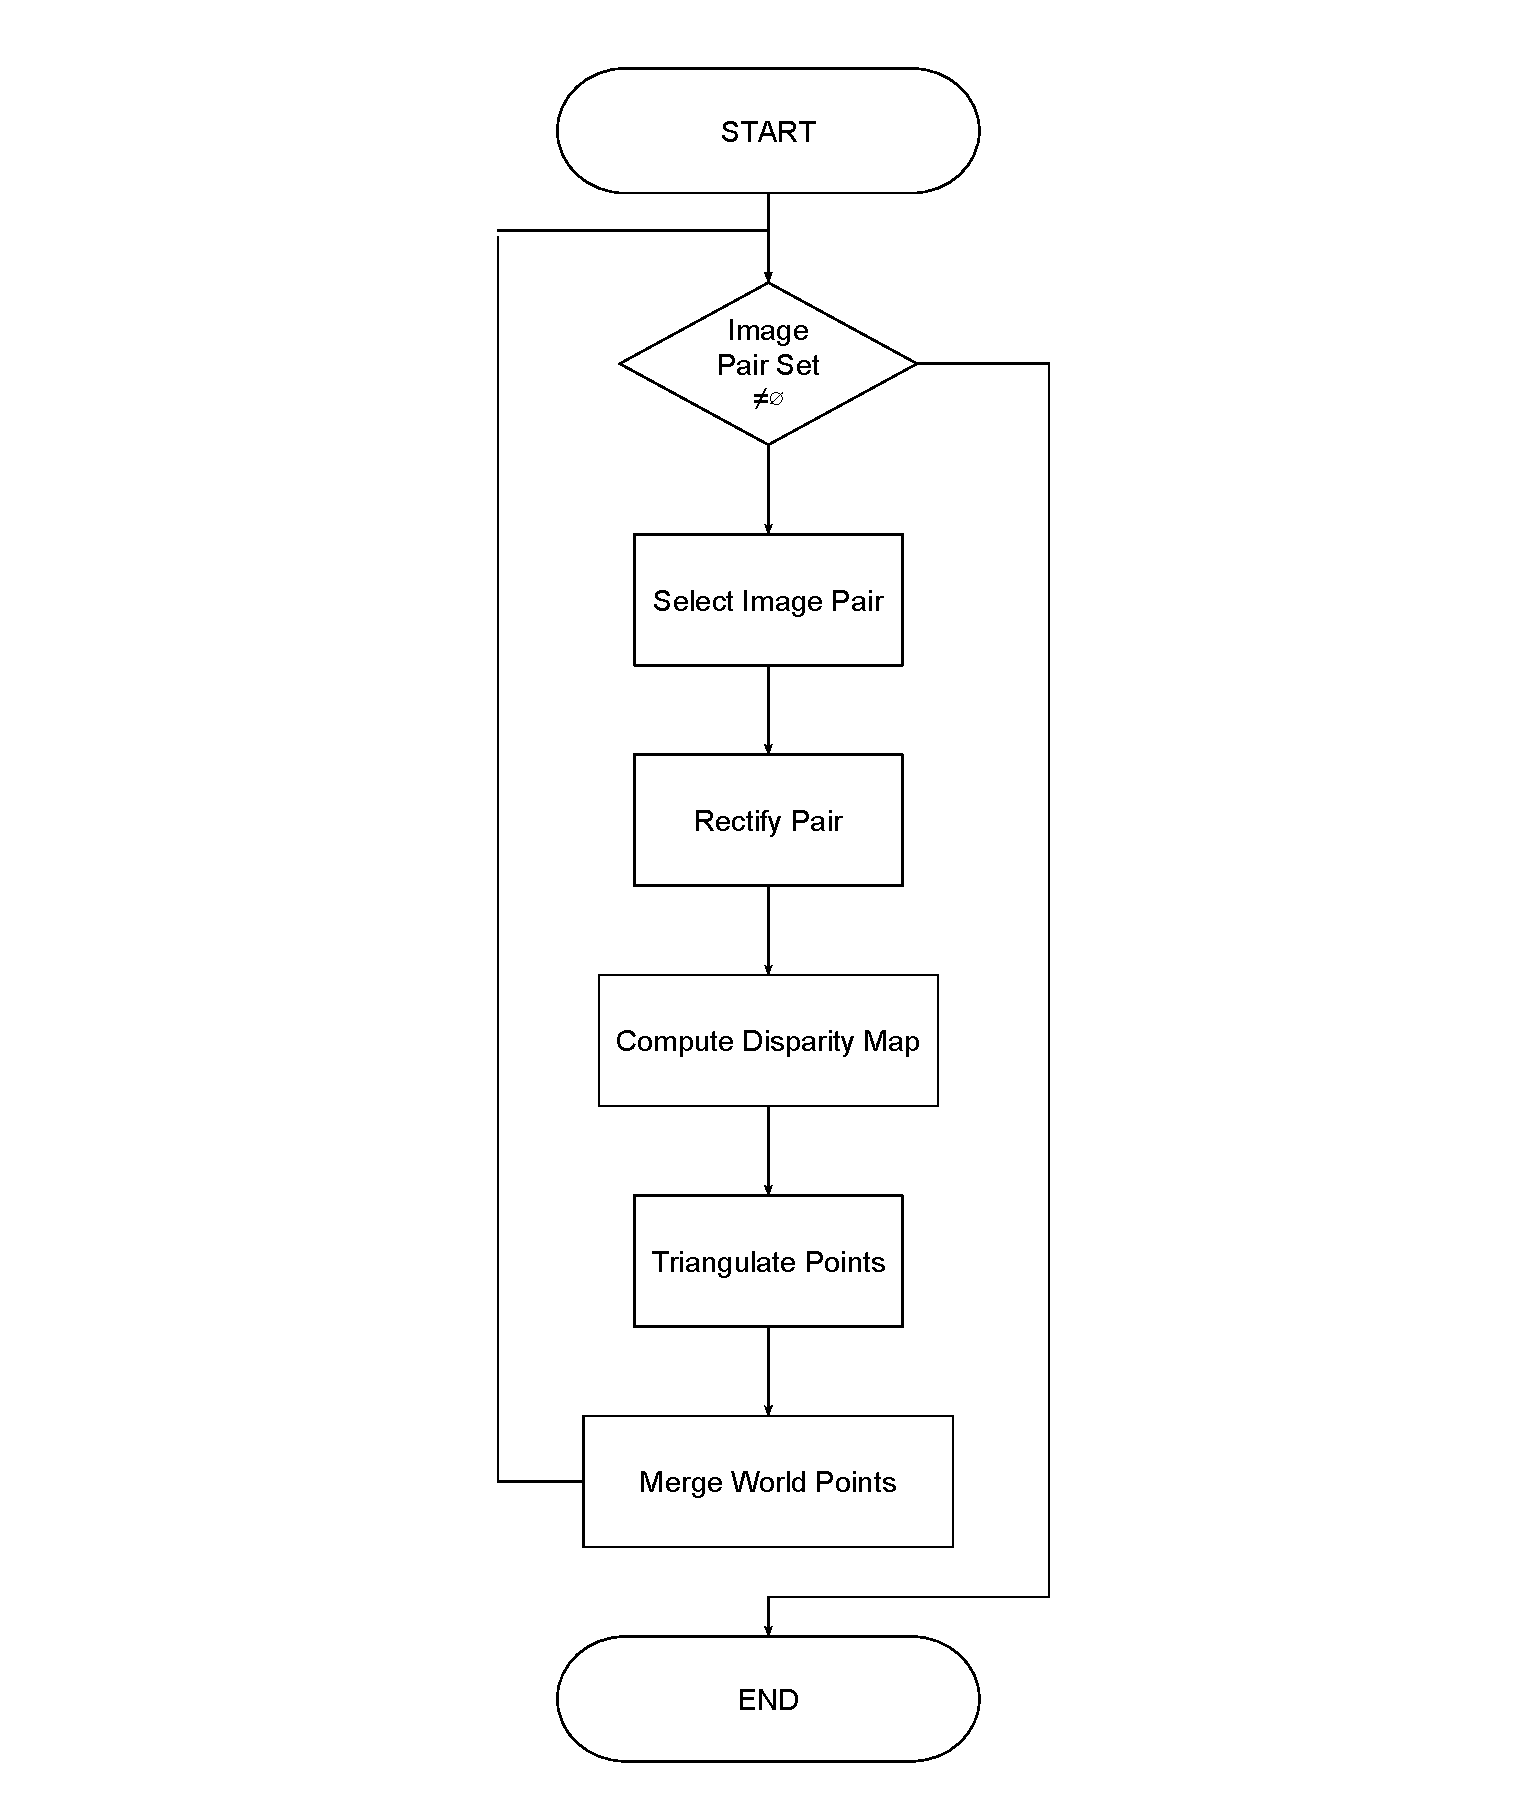
\includegraphics[width=\linewidth]{img/densification_fc.pdf}
	\caption{The flow chart representing the whole reconstruction phase.}
	\label{fig:densification_fc}
\end{figure}

\begin{figure}
	\centering
	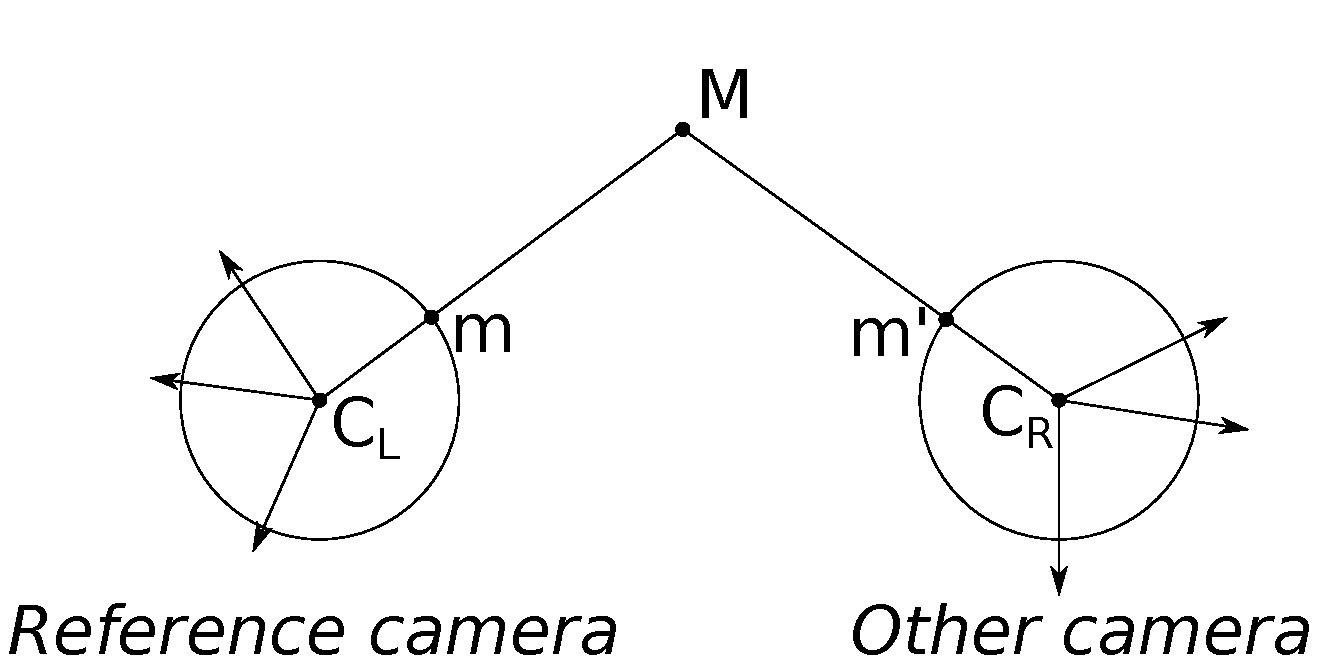
\includegraphics[width=\linewidth]{img/naming_convention.pdf}
	\caption{The naming convention used in this thesis: left camera, $C_L$,
	is the reference camera in an image pair; point $M$ is the
	\emph{world point} (see Section~\ref{subsec:triangulation}),
	and $m$ and $m^\prime$ are the two image points with respect to
	the reference and other camera respectively.}
	\label{fig:naming_convention}
\end{figure}
%
\subsection{Image Pairs Rectification}
\label{subsec:rectification}
The goal of the rectification is to transform the two images of a pair
as they were taken
with cameras whose $x$-axes were aligned along the same line and both pointing
toward the same direction, and whose $z$-axes were parallel.
With this peculiar cameras' arrangement and in case of perspective cameras,
corresponding points appears on the same row in the two rectified
images, thus the correspondences search domain is shrunk from a
2D-space to a 1D-space. In case of spherical cameras the rectification aligns
corresponding points on the same meridian, hence the same column in the two
equirectangular images.
It is important to notice that, given a point in the reference image $L$,
the possible positions that the corresponding point in the other image can
assume are always constrained to a line, even if the pair is not
rectified; these lines are called
\emph{epipolar lines}~\cite{Hartley2004,szeliski2010computer}.
Figure~\ref{fig:rectified_pair} shows the same image pair
before and after rectification.
%
\begin{figure}
	\centering
	\begin{subfigure}{0.4\linewidth}
		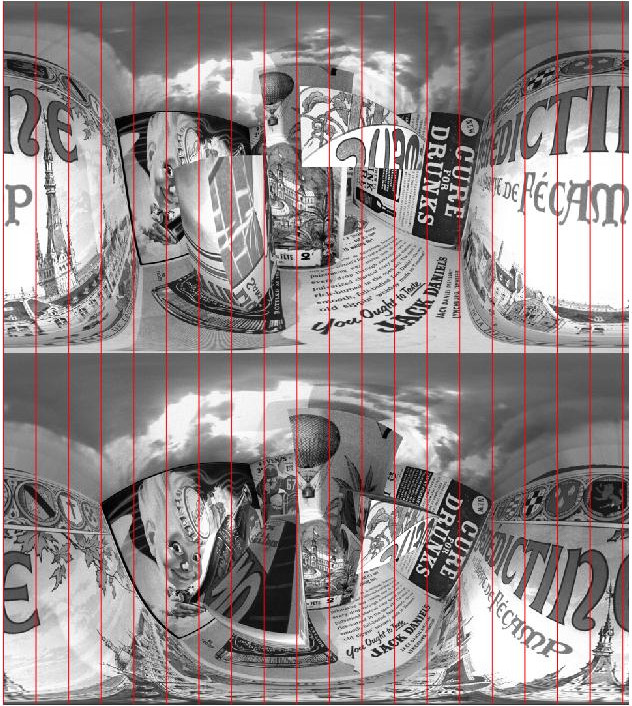
\includegraphics[width=\linewidth]{img/nonrectified_pair.jpg}
	\end{subfigure}
	\begin{subfigure}{0.4\linewidth}
		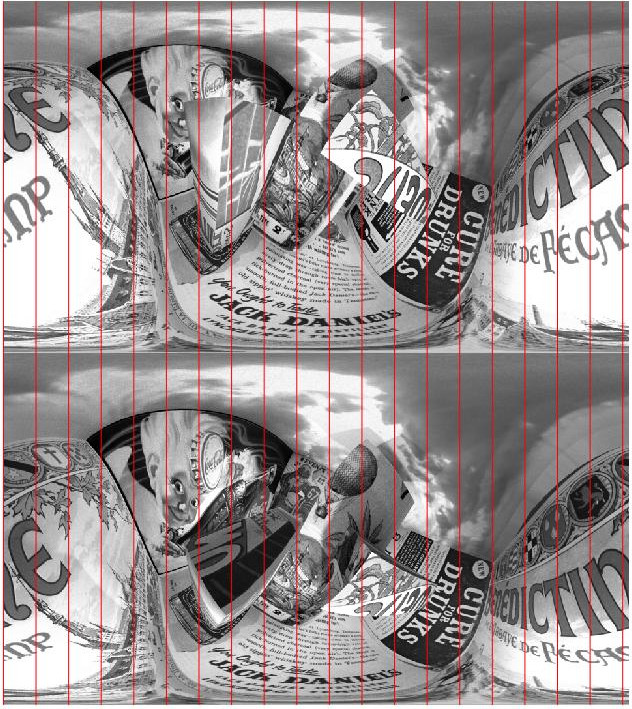
\includegraphics[width=\linewidth]{img/rectified_pair.jpg}
	\end{subfigure}
	\caption{An example of the same image pair before (left) and after
	rectification (right). Notice how, on the left of all the images,
	the corner of the letter "e" is aligned
	in the right hand pair while it is not in the left one.}\label{fig:rectified_pair}
\end{figure}

The problem is that, without rectification, the points that lie on a specific
epipolar line, have different coordinates depending on where they are on the
image sphere and, in general, they do not share the same value for any of their 
latitude or longitude angles. Thus the epipolar lines do not map to a line in
the equirectangular image, i.e. they are not represented by vertical or 
horizontal lines in this bidimensional mapping of the spherical image.
On the other hand, if the two images are rectified, all the points that lie
on an epipolar line have the same value for their longitude component, thus
they have the same horizontal coordinate in the equirectangular image.

We use the same rectification used by Ma et al. in~\cite{ma20153d} and obtain
epipolar lines that map to columns in the equirectangular image.
In particular, given an image pair, the rectification consists in a specific
rotation for each of the two cameras. Let's call $R_L$ and $R_R$ the rotation
applied to the left and right camera respectively; each rotation is obtained
by the composition of other transformations. Figure~\ref{fig:rectification} shows
the sequence of rotations we combine to obtain $R_L$ and $R_R$.
%
\begin{figure}
\centering
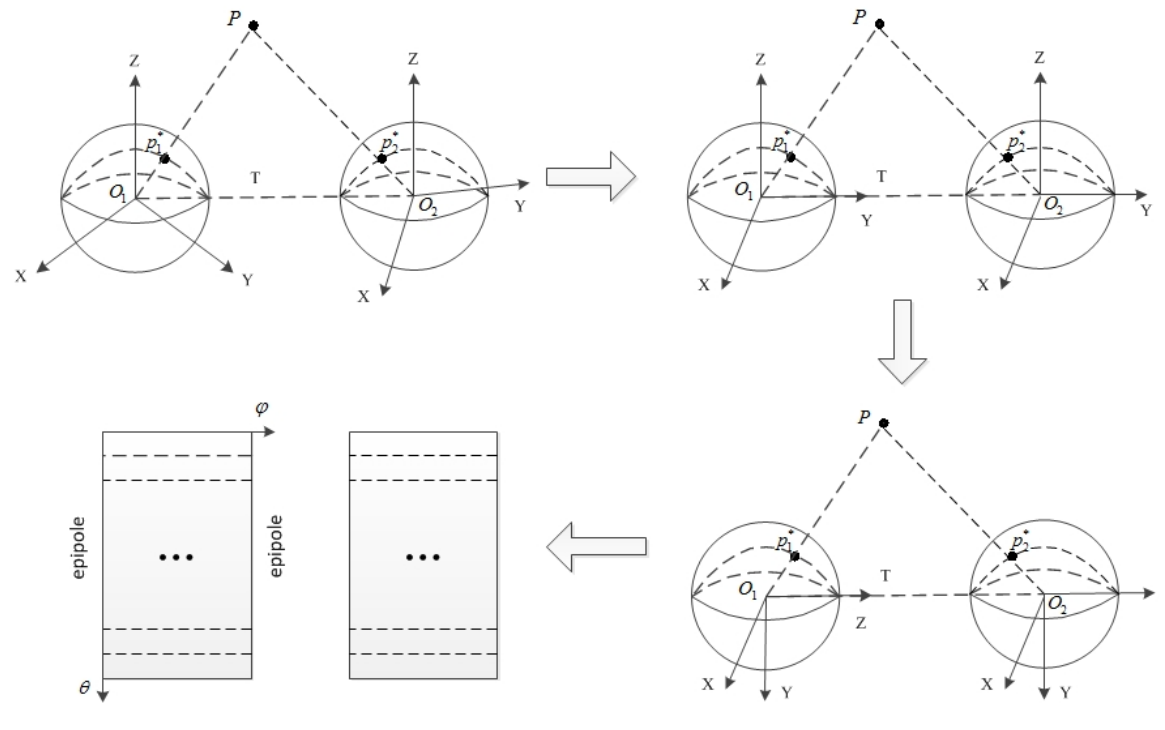
\includegraphics[width=\linewidth]{img/rectification.png}
\caption{This figure shows the transformation performed with each rotation.
First the two cameras are rotated such that their X-axes become aligned and 
their Z-axes are parallel, then a 90\degree rotation about the Z-axes aligns
the cameras' meridians to the epipolar lines. The resulting equirectangular
images have corresponding points that lie on the same column.
This picture is taken from the work of Ma et al.~\cite{ma20153d}.}
\label{fig:rectification}
\end{figure}
%
First the two rotations $R_{L, 1}$ and $R_{R, 1}$ align the two cameras' Y-axes
such that they are lie on the baseline, both pointing in the same
direction. Then $R_{R, 2}$ rotates camera $R$ around its Y-axes so that
the orientation of $R$
is the same as $L$'s. We apply one last rotation, $R_3$ to both
cameras to make them lie on a side, thus aligning the epipolar lines to the
image spheres' meridians.
Hence the overall rotations $R_L$ and $R_R$ that we must apply to cameras $L$ and $R$
respectively are:
\begin{align}
	R_L &= R_{L, 1}R_3 \\
	R_R &= R_{R, 1}R_{R, 2}R_3	\text{,}
\end{align}
\noindent where all the rotations are expressed in the post-multiplication form.

\subsection{Disparity Map Computation}
\label{subsec:disparityMap}
Given an image pair, the disparity map stores the distance in pixel between 
a point found in the reference image $L$ and its correspondence in the
other image $R$.
In case of rectified equirectangular images the disparity of a specific pixel
refers to the difference between the $v$-coordinate of the point in $L$ and the
same coordinate in $R$.
Contrary to feature matching (Section~\ref{subsec:feature_matching}), we do not
want to find the distance for few keypoints; in fact, the aim of this step is to
find the correspondence for each point that appears in the reference image.
The block-matching class of algorithms computes disparities by extracting the 
pixels surrounding a point that it wants to match and computing a similarity
or error metric with the neighbourhood pixels of each of the candidate points
in the other image. The small squared area extracted from each point is called
\emph{patch} or \emph{block}, thus the name block-matching.
There are several parameters in block-matching algorithms that affect the
resulting disparity maps; among them, there are:
\begin{itemize}
	\item \emph{patch size}: the number of pixels for each patch's side ($N$);
	\item \emph{maximum disparity}: this defines the boundaries for the search,
	i.e. how far, in pixels, the algorithm moves
	above and below the corresponding pixel in the other image
	(in the perspective case, this value refers to the
	horizontal distance traveled by the searching procedure);
	\item similarity/error metric employed: how the error or similarity metric
	is calculated.
\end{itemize}

In our pipeline, we use a block-matching algorithm with SSD error metric.
Given the two images $I_L$ and $I_R$, the SSD metric is computed as:
%
\begin{equation*}
SSD(u, v, d) = \sum_{(k, l)}(I_L(u + k, v + l) - I_R(u + k, v + l + d))^2	\textit{,}
\end{equation*}
%
\noindent where $k, l \in [-N, N]$ and $I_X(i, j)$ is the intensity level
of pixel $(i,j)$ in the gray image $X$.
%
In order to increase the matching robustness, we minimize the result of the
interpolation between the SSD response to both the original and differential 
images according to a parameter $\alpha$~\cite{BMVC.25.14:abbreviated}.
%
Then, our SSD result is given by
%
\begin{equation*}
\begin{split}
SSD(u, v, d) = (1 - \alpha) \left[ \sum_{(k, l)}(I_L(u + k, v + l) - I_R(u + k, v + l + d))^2\right] + \\
	 + \alpha\left[ \sum_{(k, l)}(I_{x,L}(u + k, v + l) - I_{x,R}(u + k, v + l + d))^2 + \right. \\
	 + \left. \sum_{(k, l)}(I_{y,L}(u + k, v + l) - I_{y,R}(u + k, v + l + d))^2 \vphantom{\sum_{(k, l)}} \right] \text{,}
\end{split}
\end{equation*}
%
\noindent where $I_{x, J}$ and $I_{y, J}$ are the differential results of image $J$
computed along the $X$ and $Y$ direction respectively.

The patch size is chosen experimentally and varies with the particular scene
we use; it is usually set to 9 or 11 pixels.
The maximum disparity is computed automatically for each pair; in particular,
we look for feature matches in the two images and compute the maximum vertical
distance between matches, then we use such a value as maximum disparity.

Since the disparity map is based on the rectification procedure, its quality
is deeply affected by the previous step's result, and rectification, in turn,
depends on the accuracy of the estimated poses. In order to compensate for
rectification errors, we try to match each point in the reference image with points that
lie on a vertical stripe instead of a single-pixel column in the other image
when we look for correspondences during the disparity map
computation. With this simple modification, we can compute disparity maps
even in presence of small rectification errors. We set the stripes' width to 3
pixels.

Yet another problem that arises when computing disparity maps is
\emph{occlusion}: objects that are far from the viewer may be covered by a
foreground object in one of the two views.
Computing the disparity of a point in the reference image that is occluded in
the other image would produce an inevitably wrong result.
To remove occluded points from the disparity map, we perform the additional
\emph{cross-checking} test~\cite{BMVC.25.14:abbreviated}.
Our cross-checking step computes two disparity maps, $M_{L,R}$ and $M_{R,L}$,
for each image pair. Each map considers a different image as reference;
in particular, $M_{X,Y}$ considers image $I_X$ as the reference and $I_Y$ as the
other image. Let's assume $M_{L,R}(i, j) = d$, then we keep only those points
that satisfy the condition:
%
\begin{equation*}
	i + M_{R, L}(i + d, j) + d< t \text{,}
\end{equation*}
%
\noindent where $t$ is a threshold in pixels that we set to 2.
Occluded points are not likely to verify the constraint above, hence they are
discarded.
\subsubsection{Patch Creation}
\label{subsubsec:patch_creation}
The disparity map computing procedure that we have described so far is not
different from an equivalent procedure for the perspective case,
with the only exception of the orientation of the epipolar lines in the
rectified pairs (that are vertical instead of horizontal).
The main difference of our reconstruction phase from the traditional ones is
in the patch creation step.
The patch is usually obtained by extracting the neighbourhood pixels of the point we want
to match, but, if we apply this method to equirectangular images, the patch retains all
the distortions introduced by the particular image format, and these can prevent
correct matching results.
Instead, we introduce a novel patch creation algorithm that removes such
distortions by projecting the pixels around the points on a plane.
In this way, we obtain a less distorted patch that we can then use in the
disparity map routine we described in the previous section.
This is especially useful when the points are close to highly distorted areas,
like the ones around the poles.

In Figure~\ref{fig:patch} we show the geometry involved in the
patch creation step. In order to create a patch, we need the actual patch size
with respect to the image sphere radius. To obtain the patch size we set the
\emph{patch resolution}, $N$, that is the length in pixels of each side of the
square patch. Then we compute the two angular
resolutions of the equirectangular image with the formulas:
%
\begin{subequations}
	\label{eq:angular_resolution}
	\begin{align}
	\sigma_u &= \frac{2\pi}{W} \\
	\sigma_v &= \frac{\pi}{H}	\text{,}
	\end{align}
\end{subequations}
%
\noindent where $W$ and $H$ are the with and height of the equirectangular
image, then we set $\sigma_{max} = max(\sigma_u, \sigma_v)$.
Given the patch resolution and the image's angular density, $\sigma_{max}$, we can
compute the actual patch size, $s$, accordingly to the formula
%
\begin{equation*}
s = 2\tan\left(\frac{N\sigma_{max}}{2}\right)
\end{equation*}
%
Once we have the patch size and its resolution, we project the point of the
spherical image on the patch itself.
When we have to compute the patch that surrounds an equirectangular image point
whose coordinates are $(\lambda,\phi)$, we position the patch's plane such that
it is tangent to the image sphere in $(\lambda, \phi)$, then we project
the point's neighbourhood pixels on the patch.
%
\begin{figure}
\centering
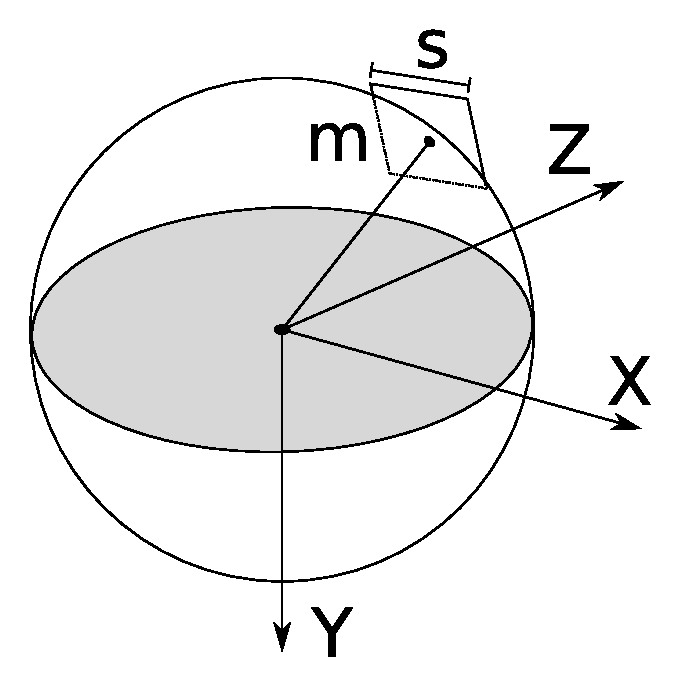
\includegraphics[width=0.7\linewidth]{img/patch_creation.pdf}
\caption{Patch creation: the neighbourhood pixels of the image point $m$
are projected on the patch. This approach prevents the patch from containing
the same distortions that are present in the equirectanguar image format.}
	\label{fig:patch}
\end{figure}
%
\subsection{World Points Triangulation}\label{subsec:triangulation}
Once we have the disparity map for a given image pair, we analyse each
disparity and compute a 3D point, the so-called \emph{world point}, for each
non-occluded point in the disparity map.
In fact, we use the disparity to obtain the image coordinates (latitude and
longitude) of the same world point as it appears in the two camera views,
thus we have the two directions where this point lies; the world point is
the intersection of these directions.
In practice, the lines defined by these two directions do not intersect
because of errors introduced by several factors (lens
distortions, image resolution, etc.). The solution is to find the mean point of the
distance between the directions and consider it as the best estimation
of the real world point's position.
Our triangulating function exploit the MATLAB's {\tt triangulateMidPoint}
that implements the solution proposed by Hartley and Sturm
in~\cite{hartley1997triangulation}. Since our matches are located on the two
image spheres, they are 3D points, thus we have to divide each of them by their
3rd component and discard it before passing them as parameters to the
MATLAB's function. This step is exactly the same that we used in order to prepare
the input parameters for the essential matrix estimation function that we
call in the camera pose estimation phase. The same considerations we made in
Section~\ref{sec:keypoints_conversion}
hold and, in particular, we do not consider those points whose
3rd component magnitude is less than a given threshold, $z_{min} = 0.01$.

The triangulated points are expressed in a reference system that has the same
orientation and position of the reference camera of the view pair.
Since the image coordinates of the matches are given for the rectified pairs,
we have to apply the inverse rotation, $R_L^\top$, in order to obtain the true
world point positions (see Section~\ref{subsec:rectification}).

\subsection{Merging World Points}\label{subsec:merging_worldPoints}
As we pointed out in the previous section, the world points are always
expressed in a reference system whose centre coincides with the reference
camera's centre of projection and that is oriented as the reference camera
itself.
Thus, in order to obtain a coherent point cloud, we have to express every world
point in a global coordinate system.
We want to merge all the point clouds obtained by the image pairs
according to the coordinate system defined
by the first view analysed. Hence, for each world point $\myvec{M}$ obtained by
an image pair whose reference camera is located at $\myvec{t}$ with orientation
$R$, we have to compute the translated point $\myvec{M}^\prime$ as
%
\begin{equation*}
\myvec{M}^\prime = R^\top \myvec{M} + \myvec{t} \text{.}
\end{equation*}
%
\noindent Once every point has been translated, the overall point cloud is
simply the union of every set of image pairs' world points.
